\documentclass[a4paper]{article}
\usepackage[utf8]{inputenc}
\usepackage{multirow}
\usepackage{graphicx}
\usepackage{a4wide}
\usepackage[pdftex,hidelinks]{hyperref}
\usepackage{float}
\usepackage{indentfirst}
\usepackage{subcaption}
\usepackage[cache=false]{minted}
\usepackage{amsmath}
\usepackage{listings}
\usepackage{color}

\begin{document}

\title{Processing an Angolan Newspaper}
\author{Pedro Mendes (a79003)}
\date{\today}

\begin{titlepage}
    \thispagestyle{empty}
    \begin{center}
        \begin{minipage}{0.75\linewidth}
            \centering
            %engenharia logo
            
\includegraphics[width=0.4\textwidth]{eng.jpeg}\par\vspace{1cm}
            \vspace{1.5cm}
            %títulos
            \href{https://www.uminho.pt/PT}
            {\scshape\LARGE Universidade do Minho} \par
            \vspace{1cm}
            \href{https://www.di.uminho.pt/}
            {\scshape\Large Departamento de Informática} \par
            \vspace{1.5cm}

            \maketitle
        \end{minipage}
    \end{center}

\end{titlepage}

\tableofcontents

\pagebreak

\section{Introduction}
This project aims to parse a very large file with articles from a newspaper in
order to organize them in individual articles, indexing them by title or tag.

The main tool used for the parser is \textit{flex}, (and the C programming
language) together with the \href{https://developer.gnome.org/}{GLib} library,
to produce an efficient parser. On top of this a \textit{bash} script was
written to pre-process the input file.

\section{The problem}

The input file presents a few challenges that need to be addressed.

The first and most obvious one is the file's size, it's millions of lines long
which means that the information parsed needs to be flushed as soon as it's not
needed anymore as to not risk allocating too much memory.

The second is the publication's format, which in some cases does not lend
itself to clean regular expressions.

\begin{figure}[H]
    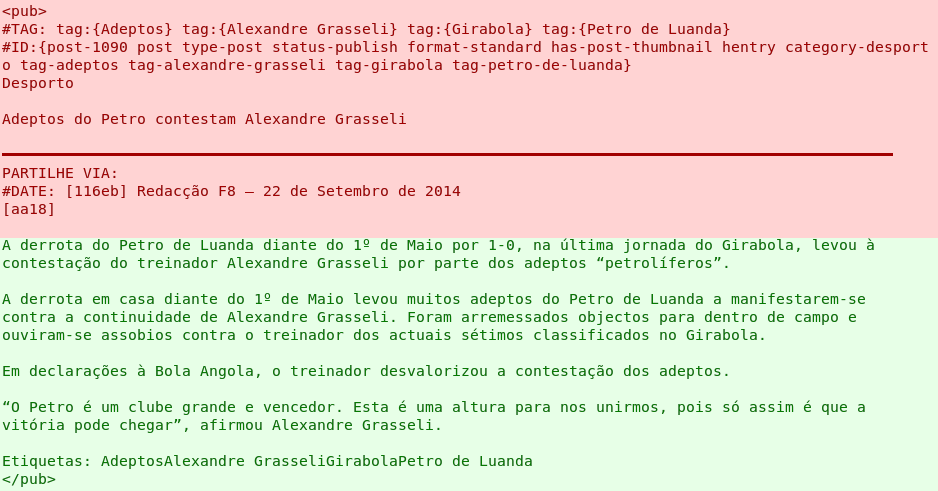
\includegraphics[width=\textwidth]{./example_pub_colored_simple.png}
    \caption{Example Publication}\label{fig:example_pub_simple}
\end{figure}

As can be seen in the example above (Figure~\ref{fig:example_pub_simple}), a
publication is split in roughly 2 parts, the header, in red, where the post's
metadata is stored and the body or text of the publication, in green. The first
area has tags, id and date which are easy to find due to their
\texttt{\#NAME\{} syntax, but the category and the title, in this example
\textit{``Desporto''} and \textit{``Adpetos de Petro contestam Alexandre
Grasseli''} respectively, have to be parsed using the rest of the header's
context. Next, sometimes there is a sequence delimited by square brackets before
the text, this is also intended to be eliminated.

The third problem to be addressed is the fact that most publications
are repeated throughout the file which can interfere with the counting of the
number of occurrences of each tag.

Lastly the fourth problem is that \textit{flex} is not unicode aware,
which means that it reads one byte at a time and since the first byte of the
horizontal bar is the same as the first byte of many other unicode characters
they are indistinguishable from \textit{flex}'s perspective. To solve this a
simple \textit{bash} script \texttt{clean\_unicode.sh} was written to replace
the horizontal bar with a sequence of \texttt{\#}.

\section{Solution}

\subsection{Parsing contexts}

To parse each publication 4 subcontexts were implemented: \textit{HEADER} (in
red), \textit{DATE} (in blue), \textit{TEXTHEADER} (in yellow) and
\textit{TEXT} (in green) (See Figure~\ref{fig:example_pub_colored}), zones in
white are ignored.

\begin{figure}[H]
    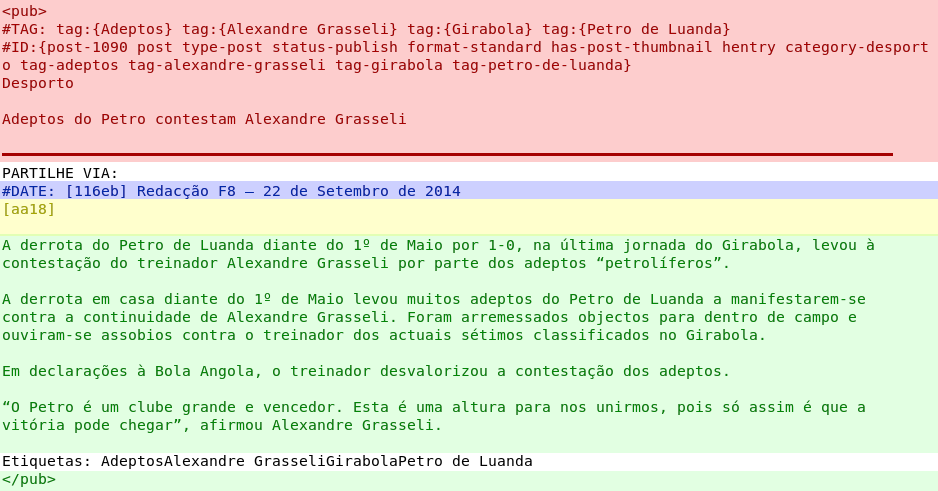
\includegraphics[width=\textwidth]{./example_pub_colored.png}
    \caption{Publication sections breakdown}\label{fig:example_pub_colored}
\end{figure}

\subsubsection{HEADER}

In the header the id, tags, category and title are parsed. The tags are
relatively easy to parse, the same goes for the id. To parse the category and
title a variable is used to know if the category has been parsed, since the
same regular expression is used for both.

\subsubsection{DATE}

The date context is started when the horizontal bar is found, and all input
strings are ignored until the \texttt{\#DATE} string is matched. At this point
the date is stored and the next context is started.

\subsubsection{TEXTHEADER}

This context serves only to remove the text between square brackets at the top
of the body, then immediately switches to the \texttt{TEXT} context.

\subsubsection{TEXT}

This context is very simple, it simply writes what it finds to the output file,
ignoring lines staring with \textit{Etiquetas:} and stopping when it finds the
end of the publication.

\section{Performance}

Program performance was a concern during it's implementation. As such for every
major feature or change made to the program time and memory benchmarks were
ran. With this system it was possible to detect a huge performance increase
when a simple change of regular expression was made.

One of regular expressions initially used was very slow and incorrect.
\begin{figure}[H]
    \centering
    \begin{verbatim}
                        AN   [0-9A-Za-zÀ-ÖØ-öø-ÿ\-]
                        ANS  [0-9A-Za-zÀ-ÖØ-öø-ÿ\- ]

                        <HEADER>{AN}{ANS}+\n
    \end{verbatim}
    \caption{First regular expression to capture the category and title}
\end{figure}

This was made in an effort to capture accented characters, but because, once
again, \textit{flex} is not unicode aware, these ranges did not work properly.
To address this, a different strategy was used, instead of listing what
characters were to be matched, we listed what characters were not to be
matched:

\begin{figure}[H]
    \centering
    \begin{verbatim}
                        <HEADER>^[^\n#<][^{\n#]+\n
    \end{verbatim}
    \caption{Correct regular expression to capture the category and title}
\end{figure}

This change cut 40\% of the programs runtime, (benchmarked from 2.5s to 1.5s)
because the list of bytes that had to be compared with was smaller. With the
added benefit of capturing more precisely titles that had unicode characters,
such as  ``,  '', --, etc.

\section{Project Architecture}

Handling of the parsed information is split in two modules,
\texttt{publication} and \texttt{newspaper}.

\subsection{Publication}

This module gathers the information of a single publication to create the
corresponding \texttt{post-id.html} file. When a publication is found this
module is initialized and, as the parser runs, this structure accumulates the
\texttt{id}, \texttt{title}, \texttt{author\_date}, \texttt{category} and
\texttt{tags}, then after the header is flushed to the post file, the body of
the publication is immediately flushed to the file as to not accumulate to many
bytes in memory.

\subsection{Newspaper}

This module indexes posts and their tags to create several files. An
\texttt{index.html} file which references all the parsed posts in a list next
to their tags. A \texttt{tags.html} file which lists all the tags found next to
their occurrence count, and finally a \texttt{<tagname>.hmtl} for every tag
which lists every file with that tag.

To achieve this two tables are kept in memory during the parsing of the whole
input string, one associates post ids with the post's title and tags, the other
associates tags with their posts. This way the relations shown below can be
achieved.

\begin{figure}[H]
    \centering
    \begin{subfigure}{0.54\textwidth}
        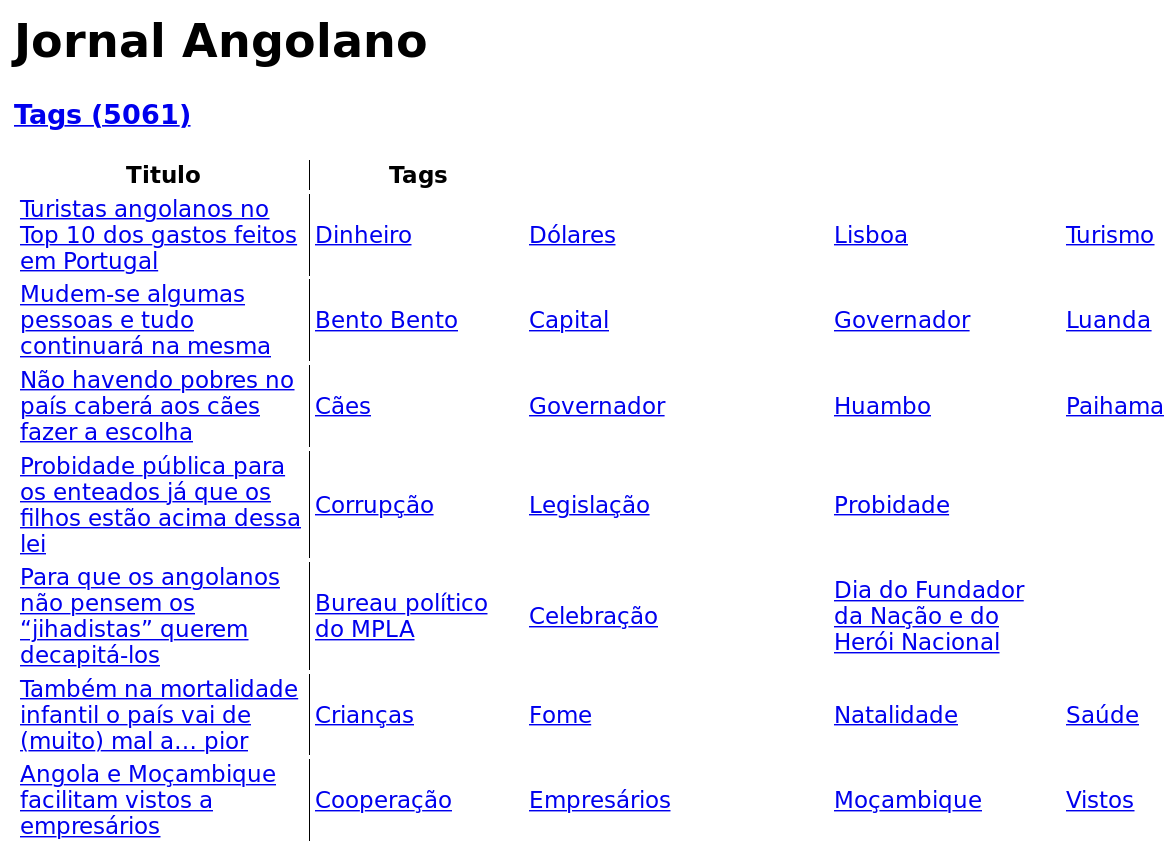
\includegraphics[width=\textwidth]{./index_print.png}
        \caption{index.html}
    \end{subfigure}
    \begin{subfigure}{0.45\textwidth}
        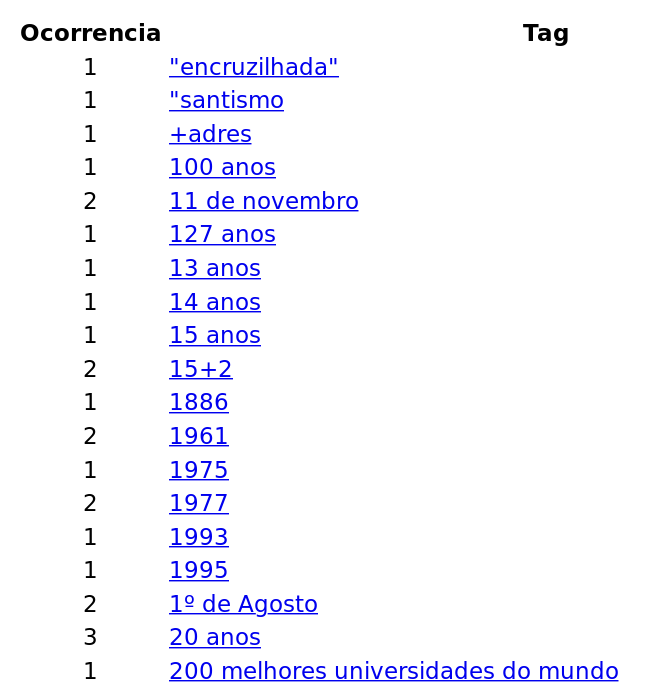
\includegraphics[width=\textwidth]{./tags_print.png}
        \caption{tags.html}
    \end{subfigure}
    \begin{subfigure}{0.45\textwidth}
        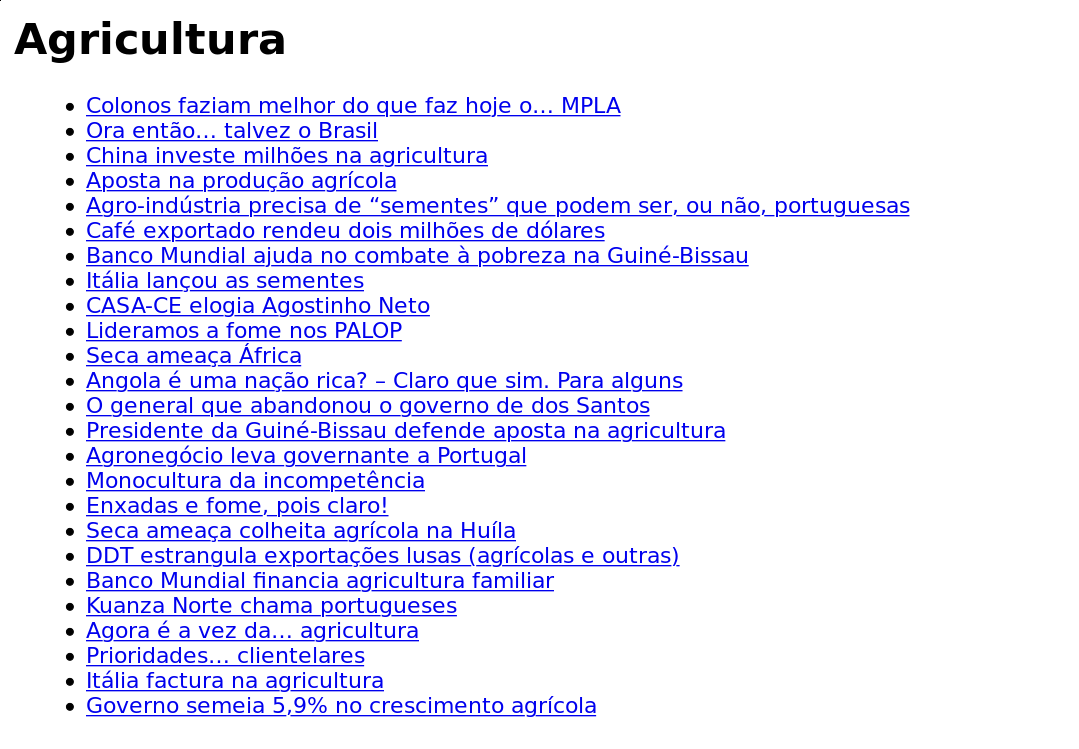
\includegraphics[width=\textwidth]{./tag_print.png}
        \caption{tag.html}
    \end{subfigure}
    \begin{subfigure}{0.54\textwidth}
        
\includegraphics[width=\textwidth]{./publication_print.png}
        \caption{publication.html}
    \end{subfigure}
    \caption{Files generated by the newspaper module}
\end{figure}

\section{Conclusion}

\end{document}

